\documentclass{article}

% \usepackage[osf]{mathpazo}
\usepackage{microtype}
\usepackage{siunitx}

\usepackage{tikz}

\usetikzlibrary
  {
    intersections,            % Name paths and intersections
    arrows,                   % extra arrow heads
    decorations.pathmorphing, % squiggly arrows
    backgrounds,              % colored background areas
    fit,                      % compute the sizes of the background areas
    positioning,              % place nodes relative to other nodes
    calc,
    through,
    shapes.misc,
  }


\begin{document}

\begin{center}
  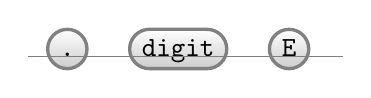
\begin{tikzpicture}
    [
      node distance=5mm,
      text height=1.5ex,
      text depth=.25ex,
      nonterminal/.style=
        {
          rectangle,
          minimum size=3ex,
          very thick,
          draw=red!50!black!50,
          top color=white,
          bottom color=red!50!black!20,
          font=\itshape,
        },
      terminal/.style=
        {
          rounded rectangle,
          minimum size=3ex,
          very thick,
          draw=black!50,
          top color=white,
          bottom color=black!20,
          font=\ttfamily,
        }
    ]
    \node (dot) [terminal] {.};
    \node (digit) [terminal, right=of dot] {digit};
    \node (E) [terminal, right=of digit] {E};

    \draw [help lines] let \p1 = (dot.base),
                           \p2 = (digit.base),
                           \p3 = (E.base)
                           in (-0.5, \y1) -- (3.5, \y1)
                              (-0.5, \y2) -- (3.5, \y2)
                              (-0.5, \y3) -- (3.5, \y3);
  \end{tikzpicture}
\end{center}

\begin{center}
  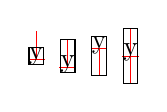
\begin{tikzpicture}[inner sep=0,node distance=.2]
    \node (y1) [draw] {y};
    \node (y2) [draw, text height=10pt, right=of y1] {y};
    \node (y3) [draw, text depth=10pt, right=of y2] {y};
    \node (y4) [draw, text height=10pt, text depth=10pt, right=of y3] {y};
    \begin{pgfonlayer}{background}
      \draw[help lines, red]
            let \p1 = (y1.base),
                \p2 = (y2.base),
                \p3 = (y3.base),
                \p4 = (y4.base)
            in (\x1, \y1) |- +(0,  10pt) ++(-3pt, 0) -- +(6pt, 0)
               (\x2, \y2) -- +(0,  10pt) ++(-3pt, 0) -- +(6pt, 0)
               (\x3, \y3) -- +(0, -10pt) ++(-3pt, 0) -- +(6pt, 0)
               (\x4, \y4) -- +(0,  10pt) ++(-3pt, 0) -- +(6pt, 0)
               (\x4, \y4) -- +(0, -10pt);
    \end{pgfonlayer}
  \end{tikzpicture}
\end{center}


\begin{center}
  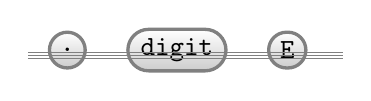
\begin{tikzpicture}
    [
      node distance=5mm,
      nonterminal/.style=
        {
          rectangle,
          minimum size=3ex,
          very thick,
          draw=red!50!black!50,
          top color=white,
          bottom color=red!50!black!20,
          font=\itshape,
        },
      terminal/.style=
        {
          rounded rectangle,
          minimum size=3ex,
          very thick,
          draw=black!50,
          top color=white,
          bottom color=black!20,
          font=\ttfamily,
        }
    ]
    \node (dot) [terminal] {.};
    \node (digit) [terminal, right=of dot] {digit};
    \node (E) [terminal, right=of digit] {E};

    \draw [help lines] let \p1 = (dot.base),
                           \p2 = (digit.base),
                           \p3 = (E.base)
                           in (-0.5, \y1) -- (3.5, \y1)
                              (-0.5, \y2) -- (3.5, \y2)
                              (-0.5, \y3) -- (3.5, \y3);
  \end{tikzpicture}
\end{center}

\begin{center}
  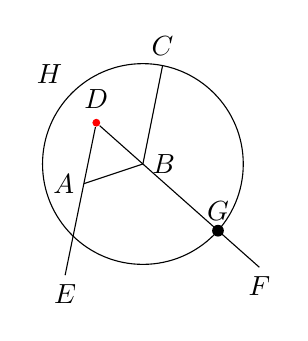
\begin{tikzpicture}
    \coordinate [label=left:$A$] (A) at (0,0);
    \coordinate [label=right:$B$] (B) at (.75,.25);
    \coordinate [label=above:$C$] (C) at (1,1.5);
    \draw (A) -- (B) -- (C);

    % \node [circle,inner sep=1pt,fill=red,label=below:$X$] (X) at ($(A)!.5!(B)$) {};
    % \node [circle,inner sep=1pt,fill=red,label=above:$D$] (D)
    %   at ($(A) ! .5 ! (B) ! 2*sin(60) ! 90:(B)$) {};

    % length of 1, rotate 60deg around (A)
    \node [circle,inner sep=1pt,fill=red,label=above:$D$] (D)
      at ($(A) ! 1 ! 60:(B)$) {};

    \node (H) [name path=H, label=135:$H$, circle through=(C), draw] at (B) {};
    \draw (D) -- ($ (D) ! 2.5 ! (A) $) coordinate [label=below:$E$] (E);
    \draw (D) -- ($ (D) ! 3.5 ! (B) $) coordinate [label=below:$F$] (F);

    \path [name path={B-F}] (B) -- (F);
    \path [name intersections={of=B-F and H, by={[label=$G$]G}}];

    % Either of these will work
    % \fill (G) circle (2pt);
    \node [fill=black,circle,inner sep=1.5pt] at (G) {};

  \end{tikzpicture}
\end{center}

\begin{center}
  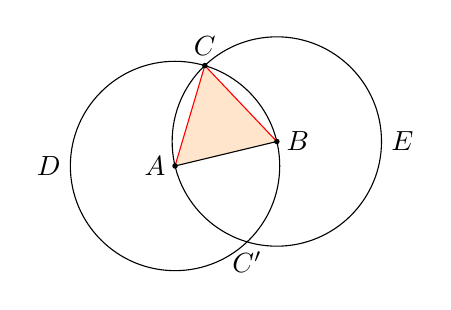
\begin{tikzpicture}
    \coordinate [label=left:$A$] (A) at ($ (0,0) + .1*(rand,rand) $);
    \coordinate [label=right:$B$] (B) at ($ (1.25, 0.25) + .1*(rand,rand) $);

    \draw (A) -- (B);
    \node (D) [draw, circle through=(B), label=left:$D$, name path=D] at (A) {};
    \node (E) [draw, circle through=(A), label=right:$E$, name path=E] at (B) {};

    \path [name intersections={of=D and E, by={C,C'}}];
    \node[above] at (C) {$C$};
    \node[below] at (C') {$C'$};

    \draw[red] (A) -- (C);
    \draw[red] (B) -- (C);

    \fill (A) circle (1pt);
    \fill (B) circle (1pt);
    \fill (C) circle (1pt);

    \begin{pgfonlayer}{background}
      \path [fill=orange!20] (A) -- (B) -- (C) -- cycle;
    \end{pgfonlayer}
  \end{tikzpicture}
\end{center}

\begin{center}
  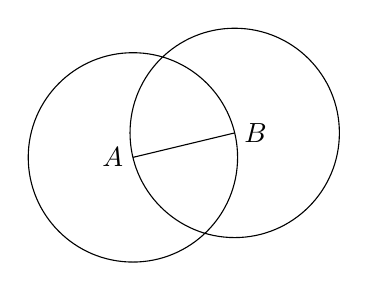
\begin{tikzpicture}
    \coordinate [label=left:$A$] (A) at ($ (0,0) + .1*(rand,rand) $);
    \coordinate [label=right:$B$] (B) at ($ (1.25, 0.25) + .1*(rand,rand) $);

    \draw (A) -- (B);
    \draw let
            \p1 = ($ (B) - (A) $), % sets x1, y1, and p1 = (x1, y1)
            \n{rad} = {veclen(\x1, \y1)}
          in
          (A) circle (\n{rad})
          (B) circle (\n{rad});
  \end{tikzpicture}
\end{center}


\begin{center}
  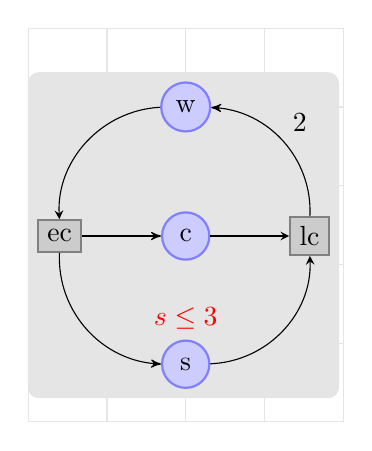
\begin{tikzpicture}
    [
      place/.style=
        {
          circle,
          draw=blue!50,
          fill=blue!20,
          thick,
          minimum size=6mm,
        },
      transition/.style=
        {
          rectangle,
          draw=black!50,
          fill=black!20,
          thick,
          minimum size=4mm,
        },
      bend angle=45,
      pre/.style={<-, >=stealth},
      post/.style={->, >=stealth'},
    ]
    \node[place]      (waiting)                            {w};
    \node[place]      (critical)       [below=of waiting]  {c};
    \node[place]      (semaphore)      [below=of critical,
                                        label={[red] above:$s \le 3$}] {s};
    \node[transition] (leave critical) [right=of critical] {lc}
      edge[pre] (critical)
      edge[post,bend right] node[auto,swap] {2} (waiting)
      edge[pre,bend left] (semaphore);
    \node[transition] (enter critical) [left=of critical]  {ec}
      edge[post] (critical)
      edge[pre,bend left] (waiting)
      edge[post,bend right] (semaphore);

    \begin{pgfonlayer}{background}
      \node
        [
          rounded corners,
          fill=black!10,
          fit=(waiting) (semaphore) (enter critical) (leave critical)
        ] {};
      \draw[color=black!10] (-2,-4) grid  (2,1);
    \end{pgfonlayer}
  \end{tikzpicture}
\end{center}

\begin{center}
  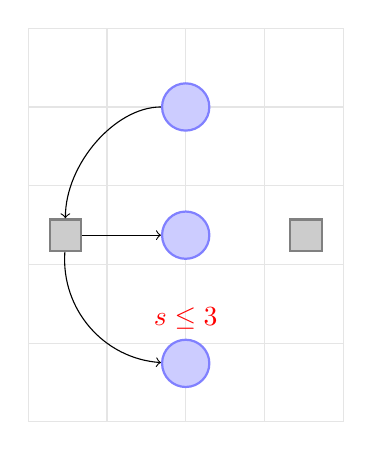
\begin{tikzpicture}
    [
      place/.style=
        {
          circle,
          draw=blue!50,
          fill=blue!20,
          thick,
          minimum size=6mm,
        },
      transition/.style=
        {
          rectangle,
          draw=black!50,
          fill=black!20,
          thick,
          minimum size=4mm,
        },
    ]
    \draw[color=black!10] (-2,-4) grid  (2,1);
    \node[place]      (waiting)                            {};
    \node[place]      (critical)       [below=of waiting]  {};
    \node[place]      (semaphore)      [below=of critical,
                                        label={[red] above:$s \le 3$}] {};
    \node[transition] (leave critical) [right=of critical] {};
    \node[transition] (enter critical) [left=of critical]  {};

    \draw [->] (enter critical) -- (critical);
    \draw [->]
      (waiting)
      .. controls +(left:.9) and +(up:.9)
      .. (enter critical);
      \draw [->] (enter critical) to [bend right=45] (semaphore);
  \end{tikzpicture}
\end{center}

\begin{center}
  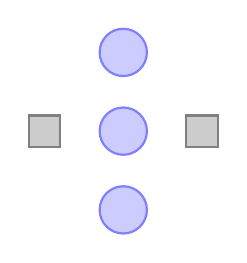
\begin{tikzpicture}
    [
      place/.style=
        {
          circle,
          draw=blue!50,
          fill=blue!20,
          thick,
          minimum size=6mm,
        },
      transition/.style=
        {
          rectangle,
          draw=black!50,
          fill=black!20,
          thick,
          minimum size=4mm,
        },
    ]
    \node[place]      (waiting 1)      at ( 0,2) {};
    \node[place]      (critical 1)     at ( 0,1) {};
    \node[place]      (semaphore)      at ( 0,0) {};
    \node[transition] (leave critical) at ( 1,1) {};
    \node[transition] (enter critical) at (-1,1) {};
  \end{tikzpicture}
\end{center}

\begin{center}
  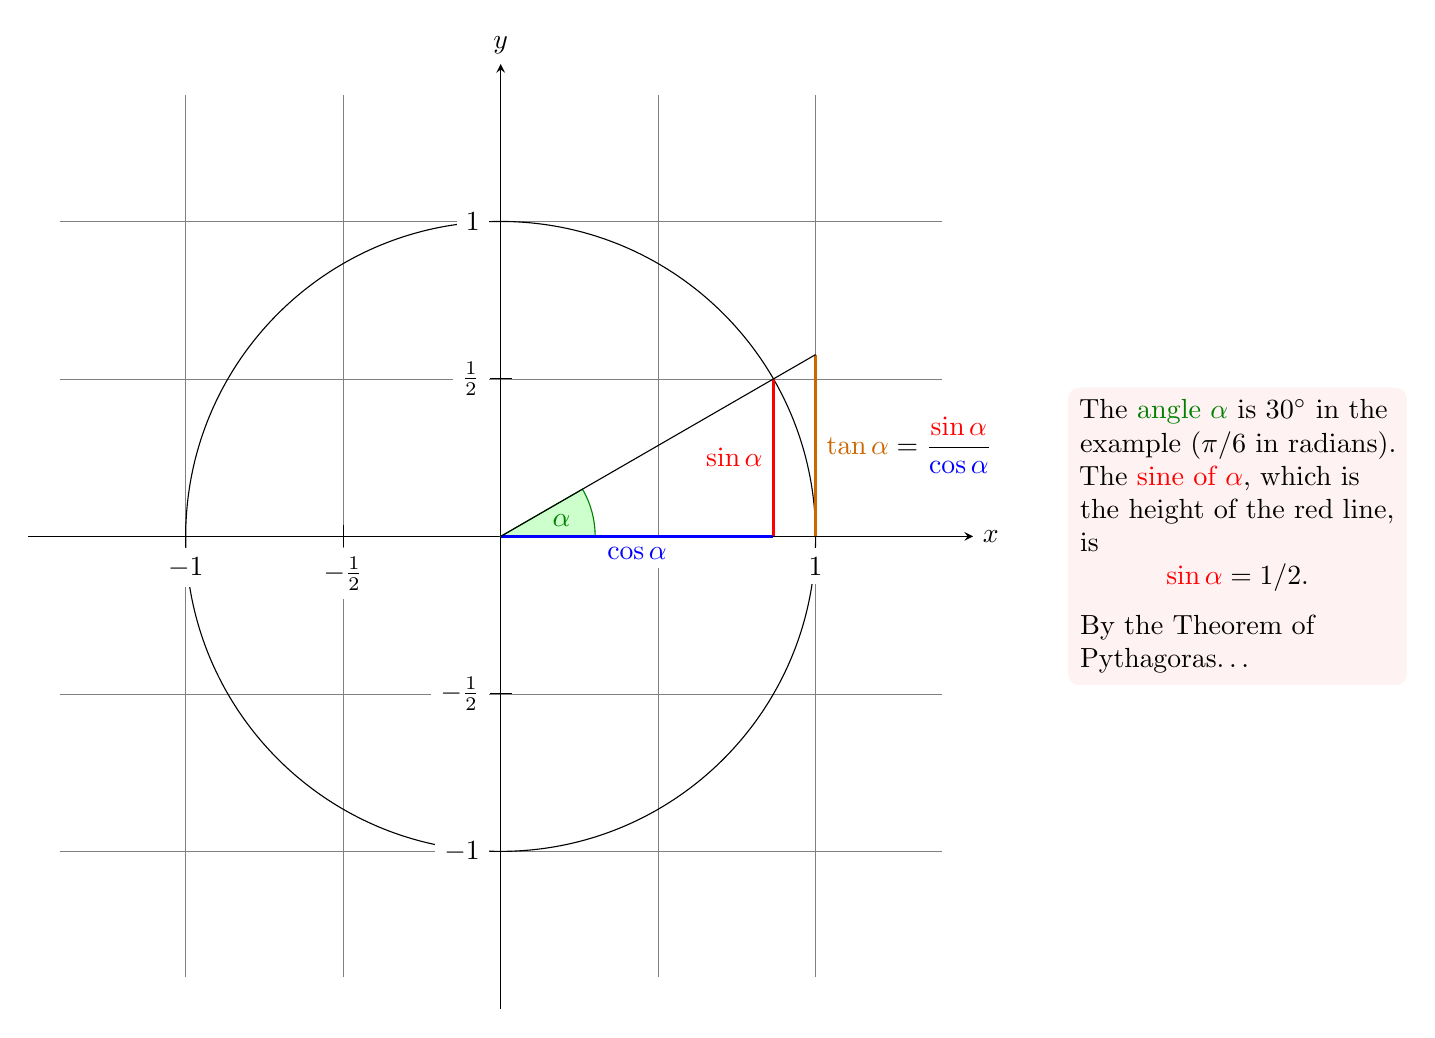
\begin{tikzpicture}
    [
      scale=4,
      % Styles
      axes/.style={>=stealth},
      important/.style={very thick},
      info text/.style={rounded corners, fill=red!5, inner sep=1ex}
    ]

    % Colors
    \colorlet{sincolor}{red}
    \colorlet{coscolor}{blue}
    \colorlet{tancolor}{orange!80!black}
    \colorlet{anglecolor}{green!50!black}
    \colorlet{anglefillcolor}{green!20!white}

    \draw [style=help lines, step=.5] (-1.4,-1.4) grid (1.4,1.4);
    \draw (0,0) circle (1);

    \begin{scope}[axes]
      \draw [->] (-1.5,0) -- (1.5,0) node [right] {$x$};
      \draw [->] (0,-1.5) -- (0,1.5) node [above] {$y$};
      % ticks
      \foreach \x/\xtext in {-1, -.5/-\frac{1}{2}, 1}
      {
        \draw [xshift=\x cm] (0, 1pt) -- (0, -1pt) node [fill=white,below] {$\xtext$};
      }
      \foreach \y/\ytext in {-1, -.5/-\frac{1}{2}, .5/\frac{1}{2}, 1}
      {
        \draw [yshift=\y cm] (1pt, 0) -- (-1pt, 0) node [fill=white,left] {$\ytext$};
      }
    \end{scope}

    \path [draw=anglecolor, fill=anglefillcolor] (0,0) -- (.3, 0) arc (0:30:.3) -- cycle;
    \draw (15:.2) node [anglecolor] {$\alpha$};

    % \draw [color=sincolor, style=very thick] (30:1) -- +(0,-0.5); % polar coords
    \draw [color=sincolor, style=important] (30:1) -- node [left,  fill=white] {$\sin \alpha$} (0,0 -| 30:1); % intersection notation
    \draw [color=coscolor, style=important]  (0,0) -- node [below, fill=white] {$\cos \alpha$} (0,0 -| 30:1);

    % named paths and intersections
    \path [name path= upward line] (1,0) -- (1,1);
    \path [name path= sloped line] (0,0) -- (30:2);
    \draw
    [
      name intersections={of=upward line and sloped line, by=pt},
      important,
      tancolor
    ]
    (1,0) --
    node [right, fill=white]
    {
      $\displaystyle
      \color{tancolor} \tan \alpha
      \color{black} =
      \frac
      {
        \color{sincolor} \sin \alpha
      }{
        \color{coscolor} \cos \alpha
      }$
    }
    (pt);

    \draw (0,0) -- (pt);

    \draw [xshift=1.8cm]
    (0,0)
    node [right, text width=4cm, info text]
    {
      The {\color{anglecolor} angle $\alpha$} is \SI{30}{\degree} in the
      example ($\pi/6$ in radians). The {\color{sincolor}sine of
      $\alpha$}, which is the height of the red line, is
      \[
        {\color{sincolor} \sin \alpha} = 1/2.
      \]
      By the Theorem of Pythagoras\ldots
    };
  \end{tikzpicture}
\end{center}

\end{document}
